\documentclass[11pt]{article}
\usepackage[margin=1in]{geometry}
\usepackage{amsmath,amssymb,amsthm}
\usepackage{graphicx}
\usepackage{booktabs}
\usepackage[hidelinks]{hyperref}
\usepackage{xcolor}

\newtheorem{theorem}{Theorem}
\newtheorem{lemma}[theorem]{Lemma}
\newtheorem{proposition}[theorem]{Proposition}
\newtheorem{corollary}[theorem]{Corollary}
\theoremstyle{definition}
\newtheorem{definition}[theorem]{Definition}
\theoremstyle{remark}
\newtheorem{remark}[theorem]{Remark}

\newcommand{\lean}[1]{\texttt{\color{black!70}#1}}
\newcommand{\R}{\mathbb{R}}

\title{The Scalar Map Theorem:\\ when rescaling a network's weights cannot change its predictions}
\author{Philip Felizarta}
\date{November 2026}

\begin{document}
\sloppy
\maketitle

\begin{abstract}
ReLU networks have a well-known symmetry: multiply a layer's weights by a positive number and the
network's predictions do not change. This note states that fact precisely, for a family of
activations we call \emph{positive scalar maps}, and extends it to networks with biases, where
the biases have to be rescaled by a specific telescoping rule. Every theorem in the note is
checked by the Lean~4 proof assistant against Mathlib, and every claim about trained networks is
reproduced by a small NumPy experiment on the scikit-learn digits data. Two practical
consequences follow. Along one of these symmetric families, top-$k$ accuracy is constant while
cross-entropy is a convex function of a single scale, so the ``best'' point is an exact
one-dimensional solve (temperature scaling), not a grid search. And a sphere in the span of three
weight vectors gives a complete picture of the accuracy over that whole span. We also correct the
protocol of our earlier experiments, which chose points on the test set: choosing on a validation
split costs 0.8 points of test accuracy on average, which is how optimistic the old numbers were.
\end{abstract}

\section{Introduction}

Take a trained classifier, multiply every weight in its first layer by 2, and divide every weight
in its last layer by 2. For a ReLU network without biases nothing observable changes: each logit
is the same, so every prediction, every accuracy and every loss is the same. Scale the first layer
by 2 and leave the rest alone, and the logits all double. The predicted class still does not
change, so accuracy is the same, but the cross-entropy does change, because softmax of doubled
logits is more confident.

This symmetry is old knowledge
\cite{neyshabur2015path,dinh2017sharp,laurent2018multilinear,lyu2020gradient,kunin2021neural}.
What this note adds is:
\begin{enumerate}
  \item An exact statement for a named class of activations (positive scalar maps,
        Definition~\ref{def:psm}), including the activations with $s(a)=a^p$, such as squared
        ReLU, and the precise rule for biases (Theorem~\ref{thm:bias}).
  \item Machine-checked proofs. The Lean names are given next to each result, and
        Section~\ref{sec:lean} explains what was checked.
  \item Two uses of the symmetry for looking at and choosing networks: a convex one-dimensional
        loss along each symmetric family (Section~\ref{sec:ray}) and complete low-dimensional
        slices of the accuracy landscape (Section~\ref{sec:slices}).
  \item Experiments that check every claim numerically, including that the theorem fails as
        soon as its assumptions fail (Section~\ref{sec:exp}).
\end{enumerate}

\section{Positive scalar maps}\label{sec:psm}

\begin{definition}[\lean{IsPSM}]\label{def:psm}
A function $g:\R\to\R$ is a \emph{positive scalar map} (PSM) with \emph{scale function}
$s:(0,\infty)\to(0,\infty)$ if
\[
  g(a x) = s(a)\, g(x) \qquad \text{for all } a>0 \text{ and all } x\in\R .
\]
\end{definition}

Only positive $a$ are allowed. Allowing all real $a$ (as in an earlier draft) would rule out ReLU,
since $\max(-x,0)\ne -\max(x,0)$. The scale function must be positive, otherwise a scaling could
flip the sign of a hidden unit, and the ordering argument below would fail.

\begin{lemma}[Examples; \lean{relu\_isPSM}, \lean{leakyReLU\_isPSM}, \lean{abs\_isPSM},
\lean{reluPow\_isPSM}, \lean{heaviside\_isPSM}]
The following are PSMs:
\begin{itemize}
  \item ReLU $\max(x,0)$, leaky ReLU or PReLU with any negative slope, $|x|$ and the identity,
        all with $s(a)=a$;
  \item $\max(x,0)^p$ for every $p\in\mathbb{N}$, with $s(a)=a^p$;
  \item the Heaviside step $\mathbf{1}[x>0]$, with $s(a)=1$.
\end{itemize}
\end{lemma}

\begin{proposition}[Structure of PSMs]\label{prop:structure}
Let $g$ be a PSM with scale function $s$.
\begin{enumerate}
  \item (\lean{IsPSM.scale\_mul}, \lean{IsPSM.scale\_one}) If $g$ is not identically zero then
        $s(ab)=s(a)s(b)$ and $s(1)=1$. With any mild regularity (for example, $s$ continuous) this
        forces $s(a)=a^p$ for some real $p$, the \emph{degree} of $g$.
  \item (\lean{IsPSM.map\_zero}) Either $g(0)=0$, or $s\equiv 1$.
  \item (\lean{IsPSM.deg1\_iff}) The PSMs with $s(a)=a$ are exactly the two-slope maps
        $g(x)=p\max(x,0)-q\max(-x,0)$.
\end{enumerate}
\end{proposition}

Part 3 says that among degree-one activations, the ReLU family is all there is. In particular no
smooth, nonlinear activation has degree one. More generally, a PSM with $s(a)=a^p$ equals
$g(1)\,x^p$ for all $x>0$, a pure power on the positive half-line. GELU, tanh, softplus, swish and
sigmoid are not, so they are not PSMs of any degree, and Section~\ref{sec:exp} shows that the
theorems below really do fail for them. (This last remark is not one of the Lean results.)

\section{The theorems}\label{sec:thm}

An MLP with $L$ layers computes
\[
  h_0=x,\qquad z_i = W_i h_{i-1} + b_i,\qquad h_i = g_i(z_i)\ (i<L),\qquad f(x)=z_L,
\]
where each hidden activation $g_i$ is applied coordinate-wise and the output $f(x)$ is the vector
of logits. In Lean this is the inductive type \lean{Net} with evaluation \lean{Net.eval}; the
indices there start at $0$, so layer $i$ here is \lean{c (i-1)} there.

\begin{theorem}[The Scalar Map Theorem; \lean{Net.scalar\_map\_theorem}]\label{thm:main}
Let $f$ be an MLP with no biases whose hidden activations are PSMs. For any positive numbers
$c_1,\dots,c_L$, let $f_c$ be the network with weights $c_i W_i$. Then there is a single number
$\beta>0$, which does not depend on the input, such that
\[
  f_c(x) = \beta\, f(x)\qquad\text{for every input } x .
\]
\end{theorem}

\begin{proof}[Proof sketch]
By induction on the layers. Suppose the input of layer $i$ has been multiplied by some $a>0$. Then
$z_i$ is multiplied by $c_i a$ (because there is no bias), and $h_i=g_i(z_i)$ is multiplied by
$s_i(c_i a)>0$ (because $g_i$ is a PSM). The final factor is
\[
  \beta = c_L\, s_{L-1}\!\Big(c_{L-1}\, s_{L-2}\big(\cdots c_2\, s_1(c_1)\cdots\big)\Big). \qedhere
\]
\end{proof}

\begin{theorem}[Biases; \lean{Net.scalar\_map\_theorem\_bias}]\label{thm:bias}
Let $f$ be an MLP, with biases, whose hidden activations are PSMs. Let $a_0=1$ and
$a_i = s_i(c_i a_{i-1})$ for $i<L$. Scale the weights by $W_i\mapsto c_iW_i$ and the biases by
\[
  b_i \mapsto c_i\, a_{i-1}\, b_i .
\]
Then the new network computes $\beta f(x)$ with $\beta = c_L a_{L-1} > 0$.
\end{theorem}

So a bias has to be scaled by everything that has already happened to its layer's input, not just
by its own layer's factor. For degree-one activations the rule is $b_i\mapsto(c_1\cdots c_i)b_i$.
Scaling each bias by $c_i$ alone (the ``naive'' rule) breaks the theorem, and so does multiplying
every parameter, weights and biases, by one number $\alpha$; both effects show up clearly in
Table~\ref{tab:invariance}.

\paragraph{Accuracy.}
Say class $y$ is in the \emph{top $k$} of a score vector $z$ when fewer than $k$ classes score
strictly higher than $y$ (\lean{InTopK}; ties count in $y$'s favour). This only depends on the order
of the scores, so it is unchanged by multiplying $z$ by a positive number (\lean{inTopK\_smul}) and
by applying softmax (\lean{inTopK\_softmax}).

\begin{corollary}[\lean{Net.topK\_count\_scaleW}, \lean{Net.topK\_count\_scale},
\lean{Net.topK\_softmax\_scale}]
Under the scalings of Theorem~\ref{thm:main} or Theorem~\ref{thm:bias}, every example keeps its
top-$k$ status, for every $k$, whether read off the logits or the softmax probabilities. Top-$k$
accuracy on any finite data set is therefore exactly the same.
\end{corollary}

\begin{corollary}[Degree one; \lean{Net.eval\_scaleW\_deg1}, \lean{Net.eval\_scaleW\_const}]
If every hidden activation has $s(a)=a$ (ReLU, leaky ReLU, PReLU, $|x|$), then
$\beta=c_1c_2\cdots c_L$. In particular, multiplying every weight of a bias-free network by
$\alpha>0$ multiplies the logits by $\alpha^L$.
\end{corollary}

\paragraph{The symmetry is bigger than one scale per layer.}
For degree-one activations each hidden unit can be rescaled on its own.

\begin{proposition}[Per-unit rescaling; \lean{Net.neuron\_rescale}]\label{prop:neuron}
Let hidden layer $i$ have a degree-one PSM activation, and let $d_j>0$ for each unit $j$ of that
layer. Multiply unit $j$'s incoming weights and bias by $d_j$ and its outgoing weights by $1/d_j$.
The network computes exactly the same function.
\end{proposition}

The functions computed are identical, not just proportional, so the loss is unchanged too. A
network with hidden widths $n_1,\dots,n_{L-1}$ therefore sits in a family of
$n_1+\cdots+n_{L-1}$ positive parameters of networks with identical outputs, plus one more for the
overall logit scale. For our $64$--$100$--$100$--$100$--$10$ networks that is $301$ free
parameters, compared with the $4$ of per-layer scaling. Per-layer scaling is the special case where
$d$ is constant on each layer, combined with the overall scale. This is the rescaling symmetry used by Path-SGD
\cite{neyshabur2015path} and in the sharpness argument of Dinh et al.~\cite{dinh2017sharp}.

\section{One dimension of loss: temperature scaling}\label{sec:ray}

Fix a bias-free degree-one network with logits $z(x)$ and walk along the ray $\alpha\theta$,
$\alpha>0$. By the degree-one corollary the logits are $t\,z(x)$ with $t=\alpha^L$, so accuracy is
constant and the mean cross-entropy is
\[
  \mathcal{L}(t) = \frac1n\sum_{d=1}^n\Big(\log\sum_j e^{t z_j(x_d)} - t z_{y_d}(x_d)\Big).
\]
\begin{proposition}\label{prop:convex}
$\mathcal{L}$ is convex in $t$, with
$\mathcal{L}'(t)=\frac1n\sum_d\big(\mathbb{E}_{p_d}[z]-z_{y_d}\big)$ and
$\mathcal{L}''(t)=\frac1n\sum_d\mathrm{Var}_{p_d}[z]\ge0$, where $p_d=\mathrm{softmax}(t z(x_d))$.
\end{proposition}

This is the standard computation behind temperature scaling \cite{guo2017calibration}; the scale
$t$ is an inverse temperature. (It is proved here on paper, not in Lean.) Two consequences:
\begin{itemize}
  \item The best point on the ray is found by a few steps of Newton's method on a validation set,
        to machine precision. The 400-point grid search in our earlier notebook found the same
        point to two decimal places (Table~\ref{tab:ray}).
  \item The loss reduction along the ray is a \emph{calibration} gain, not a generalisation gain:
        the classifier's decisions are identical everywhere on the ray. An earlier draft suggested
        that overfitting ``at large weight norm'' is explained by over-confident softmax outputs.
        Along a ray that is exactly what happens to the loss, but by construction it cannot
        explain any change in accuracy.
\end{itemize}
$\mathcal{L}$ need not be convex in $\alpha$ itself, since $t=\alpha^L$; the convexity is in $t$.

\section{Complete slices of the accuracy landscape}\label{sec:slices}

Loss-landscape plots \cite{li2018visualizing} show the loss on a plane through a trained network,
spanned by two random directions with careful (filter-wise) normalisation. For accuracy, and for a
bias-free network with PSM activations, there is a cleaner option.

Take two weight vectors $u,v$ and the closed curve $\gamma(s)=\cos(s)\,u+\sin(s)\,v$. If $u,v$ are
linearly independent, $\gamma$ is an ellipse around the origin, and every ray from the origin in
the plane $\mathrm{span}(u,v)$ meets it exactly once. By Theorem~\ref{thm:main} every point of that
ray has the same accuracy. So the accuracy along the one-dimensional curve $\gamma$ is the accuracy
on the \emph{entire} plane, except the origin. With three vectors, the surface
$\sin\phi\cos\theta\,u+\sin\phi\sin\theta\,v+\cos\phi\,w$ does the same for a three-dimensional
span.

Two points matter in practice. First, the whole curve or sphere is needed, not just the positive
quadrant: $-u$ is a different network from $u$, since leaky ReLU is not odd. Second, if a point
is \emph{chosen} from the slice, it must be chosen on data that will not be used to report the
result. Our earlier notebook chose both the direction and the scale on test examples.

\section{Experiments}\label{sec:exp}

All experiments use the scikit-learn \texttt{digits} data ($8\times8$ images, 10 classes), split
60/20/20 into train, validation and test sets ($360$ test images), and $64$--$100$--$100$--$100$--$10$
MLPs trained with Adam in float64 NumPy. They run in about a minute on a CPU
(\texttt{python/experiments/run\_all.py}). The property tests in \texttt{python/tests} check the
same statements on random networks (71 tests).

\paragraph{Invariance.} For each network we draw $200$ random per-layer scalings $c_i$,
log-uniform in $[0.1,10]$, and record how much test accuracy moves
(Table~\ref{tab:invariance}). Wherever a theorem applies, top-1 and top-3 accuracy do not move at
all, and the logits match $\beta f(x)$ to about $10^{-15}$ relative error, which is
floating-point round-off. Wherever an assumption is broken (the naive bias rule, scaling biases
and weights by one $\alpha$, or a non-PSM activation) accuracy moves, in some cases by most of its
range. Per-unit rescaling of all three hidden layers of the biased ReLU network (factors
log-uniform in $[0.1,10]$) changed no logit by more than $1.4\times10^{-14}$.

\begin{table}[t]
\centering
\begin{tabular}{lccc}
\toprule
Network and scaling rule & test acc. & top-1 range & top-3 range \\
\midrule
Leaky ReLU (0.3), no bias (Thm.~\ref{thm:main}) & 0.972 & 0 & 0 \\
ReLU, no bias (Thm.~\ref{thm:main}) & 0.981 & 0 & 0 \\
ReLU, biases, telescoping rule (Thm.~\ref{thm:bias}) & 0.983 & 0 & 0 \\
ReLU$^2$, biases, telescoping rule (Thm.~\ref{thm:bias}, $s(a)=a^2$) & 0.911 & 0 & 0 \\
\midrule
ReLU, biases, naive rule $b_i\mapsto c_ib_i$ & 0.983 & 0.733 & 0.525 \\
ReLU, biases, all parameters $\times\,\alpha$ & 0.983 & 0.900 & 0.617 \\
GELU, no bias & 0.981 & 0.194 & 0.011 \\
tanh, no bias & 0.986 & 0.033 & 0.006 \\
softplus, no bias & 0.972 & 0.861 & 0.706 \\
\bottomrule
\end{tabular}
\caption{Range (max $-$ min) of test accuracy over $200$ random per-layer scalings. Above the line
the assumptions of a theorem hold; below it one is broken. ``test acc.'' is the unscaled network.}
\label{tab:invariance}
\end{table}

\paragraph{The ray.} Figure~\ref{fig:ray} shows cross-entropy and accuracy along $\alpha\theta$ for
the bias-free leaky ReLU network. Accuracy is a flat line; the loss has a single minimum, found by
Newton's method on the validation set (Table~\ref{tab:ray}). The gain is small here because Adam
had already reached a reasonable temperature, but the computation is exact and costs a handful of
forward passes.

\begin{figure}[t]
\centering
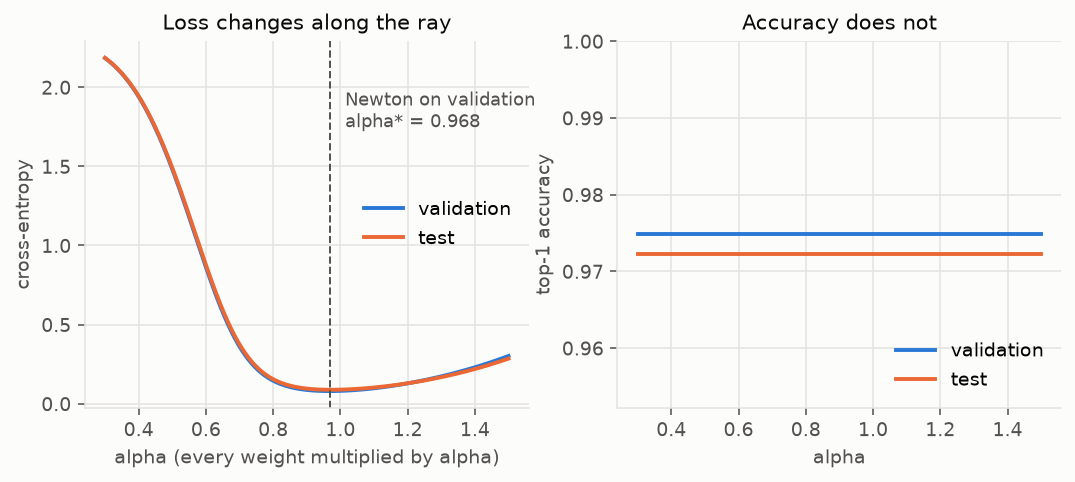
\includegraphics[width=\linewidth]{../results/exp2_ray.png}
\caption{Along the ray $\alpha\theta$ of a bias-free leaky ReLU network, cross-entropy changes and
accuracy does not.}
\label{fig:ray}
\end{figure}

\begin{table}[t]
\centering
\begin{tabular}{lccc}
\toprule
 & $\alpha$ & val.\ CE & test CE \\
\midrule
Trained network & 1 & 0.0810 & 0.0886 \\
Grid search, 400 points (old notebook, here on validation) & 0.970 & 0.07977 & -- \\
Newton on $t=\alpha^4$, validation & 0.9677 & 0.07976 & 0.0879 \\
\bottomrule
\end{tabular}
\caption{Choosing the scale. Test accuracy is $0.972$ in every row, by Theorem~\ref{thm:main}.}
\label{tab:ray}
\end{table}

\paragraph{Slices.} Following the earlier notebook, we take the initial weights $w_0$ and
snapshots $m_1$ (after one epoch) and $m_2$ (after six) of a bias-free leaky ReLU network, and
evaluate the sphere $x w_0+y m_1+z m_2$ on a $72\times36$ grid (Figure~\ref{fig:sphere}). The
earlier protocol picks the best point on the test set and reports test accuracy there; ours picks
on validation. Over five seeds, the old protocol reports $0.968$ mean test accuracy and ours
$0.960$, the same as the final snapshot ($0.961$). The $0.8$-point gap is the optimism of
selecting on test data. On this small problem, searching the sphere found nothing better than
training on.

\begin{figure}[t]
\centering
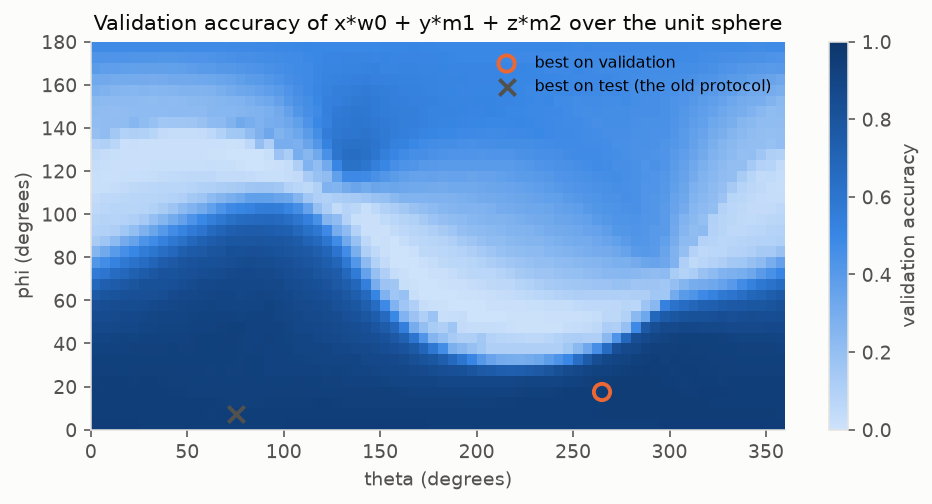
\includegraphics[width=\linewidth]{../results/exp3_sphere.png}
\caption{Validation accuracy over the sphere spanned by $w_0$, $m_1$, $m_2$ (seed 0). By
Theorem~\ref{thm:main} this is the accuracy on the whole three-dimensional span.}
\label{fig:sphere}
\end{figure}

\begin{figure}[t]
\centering
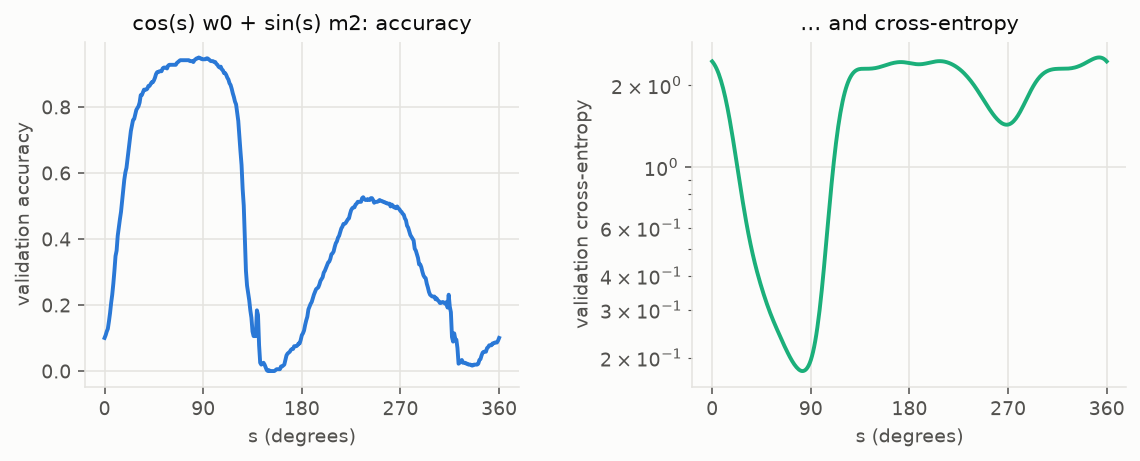
\includegraphics[width=\linewidth]{../results/exp3_circle.png}
\caption{The one-dimensional version: $\cos(s)w_0+\sin(s)m_2$ covers the whole plane of $w_0$ and
$m_2$. Note that $s$ and $s+180^\circ$ differ: $-m_2$ is a different network.}
\label{fig:circle}
\end{figure}

\section{What Lean checked}\label{sec:lean}

The \texttt{lean/} directory is a Lake project pinned to Lean~4 (\texttt{v4.37.0-rc1}) and the
matching Mathlib \cite{demoura2021lean4,mathlib2020}. Networks are an inductive type of affine
layers over real-valued vectors indexed by \texttt{Fin n}, of arbitrary depth and widths, with an
activation (and its scale function and PSM proof) attached to each hidden layer. Every result
labelled with a Lean name above is proved there, with no \texttt{sorry}; \texttt{lean/Axioms.lean}
prints the axioms each headline theorem depends on, and they are only Lean's three standard ones
(\texttt{propext}, \texttt{Classical.choice}, \texttt{Quot.sound}).

What is \emph{not} in Lean: the convexity of Proposition~\ref{prop:convex}, the claim that GELU and
the other smooth activations are not PSMs, the ``every ray meets the ellipse once'' argument of
Section~\ref{sec:slices}, and of course the experiments. The Lean model uses exact real arithmetic;
the experiments use float64.

\section{Related work}

The positive rescaling symmetry of ReLU networks is well known. Neyshabur, Salakhutdinov and
Srebro \cite{neyshabur2015path} design an optimiser (Path-SGD) that is invariant to it; Dinh et
al.~\cite{dinh2017sharp} use it to show that sharpness-based measures of generalisation can be
changed arbitrarily without changing the function; Laurent and von Brecht
\cite{laurent2018multilinear} study the multilinear structure it induces; Lyu and Li
\cite{lyu2020gradient} analyse gradient descent on homogeneous networks; and Kunin et
al.~\cite{kunin2021neural} derive conservation laws from it. Li et al.~\cite{li2018visualizing}
introduce filter-wise normalisation for loss-landscape plots precisely because of this scale
dependence. Temperature scaling \cite{guo2017calibration} is the calibration method that the
one-dimensional loss solve of Section~\ref{sec:ray} reduces to. Our contribution is the exact
statement for general PSMs with biases, its formal verification, and the two uses of it in
Sections~\ref{sec:ray} and~\ref{sec:slices}.

\begin{thebibliography}{99}\small
\bibitem{demoura2021lean4} L.~de Moura and S.~Ullrich. The Lean 4 theorem prover and programming
  language. \emph{CADE}, 2021.
\bibitem{dinh2017sharp} L.~Dinh, R.~Pascanu, S.~Bengio and Y.~Bengio. Sharp minima can generalize
  for deep nets. \emph{ICML}, 2017.
\bibitem{guo2017calibration} C.~Guo, G.~Pleiss, Y.~Sun and K.~Q.~Weinberger. On calibration of
  modern neural networks. \emph{ICML}, 2017.
\bibitem{kunin2021neural} D.~Kunin, J.~Sagastuy-Brena, S.~Ganguli, D.~L.~K.~Yamins and
  H.~Tanaka. Neural mechanics: symmetry and broken conservation laws in deep learning dynamics.
  \emph{ICLR}, 2021.
\bibitem{laurent2018multilinear} T.~Laurent and J.~von Brecht. The multilinear structure of ReLU
  networks. \emph{ICML}, 2018.
\bibitem{li2018visualizing} H.~Li, Z.~Xu, G.~Taylor, C.~Studer and T.~Goldstein. Visualizing the
  loss landscape of neural nets. \emph{NeurIPS}, 2018.
\bibitem{lyu2020gradient} K.~Lyu and J.~Li. Gradient descent maximizes the margin of homogeneous
  neural networks. \emph{ICLR}, 2020.
\bibitem{mathlib2020} The mathlib Community. The Lean mathematical library. \emph{CPP}, 2020.
\bibitem{neyshabur2015path} B.~Neyshabur, R.~Salakhutdinov and N.~Srebro. Path-SGD:
  path-normalized optimization in deep neural networks. \emph{NeurIPS}, 2015.
\end{thebibliography}

\end{document}
